%%%%%%%%%%%%%%%%%%%%%%%%%%%%%%%%%%%%%%%%%%%%%%%%%%%%%%%%%%%%%%%%%%%%
% Ergebnis
%%%%%%%%%%%%%%%%%%%%%%%%%%%%%%%%%%%%%%%%%%%%%%%%%%%%%%%%%%%%%%%%%%%%

\chapter{Ergebnis}
  \label{Ergebnis}

Eine funktionierende Orientierung lässt sich bereits mit dem Azimut-Wert des Kompasses und dem Elevation-Wert, den das Gyroskop liefert, realisieren. Allerdings ist diese Anordnung sehr anfällig auf Deviation. Deviation ist eine Ablenkung eines Magnetkompasses, die mit elektromagnetischen Feldern in der Umgebung des Kompasses zusammenhängt. Außerdem sind die Werte des Kompasses, vor allem in älteren iOS Versionen, sehr sprunghaft. 

Eine weitere funktionierende Möglichkeit besteht darin, den Kompass nur für den initialen Azimut-Wert heranzuziehen. Alle weiteren Änderungen können vom Gyroskop bestimmt werden. Jedoch hat sich in Tests ergeben, dass der Drift des Gyroskops so stark ist, dass nach wenigen Sekunden eine inakzeptable Abweichung vom korrekten Wert errechnet wird. Eine Idee war, den Gyroskop-Wert an den Kompass-Wert anzugleichen wenn das Gerät eine bestimmte Zeit lang in Ruhe war. Jedoch entsteht so immer einen Sprung wenn die Angleichung stattfindet. In der fertigen App würde das einen plötzlichen Bildausschnittssprung zur Folge haben. Dieser wäre für den Benutzer nicht nachvollziehbar.

\begin{figure}[htb]
\centering
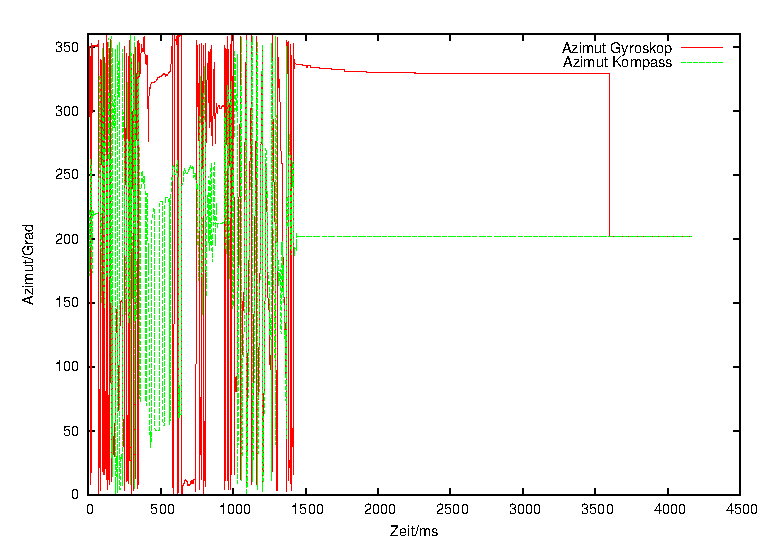
\includegraphics[scale=1]{figures/heading004}
\caption{Azimut-Wert des Gyroskops im Vergleich zum Azimut-Wert des Kompasses}
\label{fig:heading004}
\end{figure}

In Grafik \ref{fig:heading004} wird der Azimut-Wert des Kompasses in grün angegeben. Die Messung wurde in einer Umgebung durchgeführt, in der keine Magnetfeld-Störungen ermittelt werden konnten. Das iPad wurde über eine Dauer von $1500ms$ schnell in beliebige Orientierungen bewegt. Danach war es in Ruhe. Nach einer Phase der schnellen Orientierungsänderung weicht der mit Daten des Gyroskops ermittelte Azimut-Wert (rot) fast $150^o$ vom Kompass-Azimut ab. Diese Abweichung ist eindeutig zu hoch. Man erkennt auch nach ca. $3600ms$ den Angleichungssprung. In diesem Moment würde sich das 3D-Modell auf dem Gerät um $150^o$ drehen. Diese Grafik ist das Resultat einer einzigen Messung, also nciht allgemein gültig. Aber es sie zeigt, dass mindestens einer der beiden Sensoren falsche Daten liefern kann. Der Azimut-Wert des Kompasses zeigt gelegentlich Sprünge, der des Gyroskops wird schnell sehr ungenau. Es muss also eine Fusion stattfinden um einen möglichst genauen Wert zu erzielen.

\begin{figure}[htb]
\centering
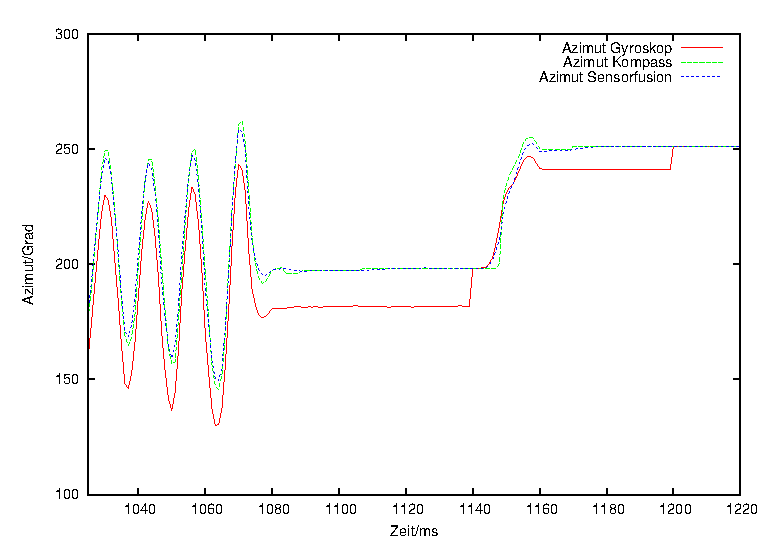
\includegraphics[scale=1]{figures/heading003}
\caption{Azimut berechnet durch Sensorfusion}
\label{fig:heading003}
\end{figure}

In Grafik \ref{fig:heading003} wird die Multisensordatenfusion (blau) mit dazu genommen – wieder in der selben Umgebung. Es ist zu erkennen, dass sie deutlich näher am Wert des Kompasses liegt. Die Kompassbewegungen werden durch die Multisensordatenfusion geglättet, sodass eine sanfte Bewegung des 3D-Modells entsteht, ohne zu stark von der realen Bewegung des Geräts abzuweichen. Diese Messung wurde mit den Steuerungsvariablen \texttt{phi} $=1$ und \texttt{alpha} $=19$ vorgenommen. In Tests hat sich das Mischungsverhältnis von 1:19 bewährt. Bei einem Verhältnis von ca. 1:10, also einem höheren Kompass-Anteil, ist die Glättung der Sprünge des Kompasses durch den Azimut-Wert des Gyroskops nicht groß genug. Bei einem wesentlich höheren Anteil des Gyroskopswerts mit einem Mischungsverhältnis von ca. 1:80 ist die Fehlerkorrektur in der Ruhe zu sehr bemerkbar. Die Driftkorrektur durch den Azimut-Wert des Kompasses ist in diesem Fall nicht groß genug. Wenn das Gerät schnell bewegt wird summieren sich Rechenfehler. Die Korrektur kann wegen den schnellen Bewegungen nicht zum Tragen kommen. Wenn das Gerät danach in Ruhe ist, kann man beobachten wie sich die Orientierung wieder langsam dem korrekten Wert annähert. Dies sollte aber im Optimalfall nicht zu sehen sein. Nur Bewegungen die tatsächlich stattfinden, sollten auch im 3D-Modell sichtbar sein. So findet eine als unnatürlich wahrgenommene Bewegung statt, wodurch die Synchronisierung zwischen Realität und 3D-Modell auf dem Gerät für den Benutzer verloren geht.

\begin{figure}[htb]
\centering
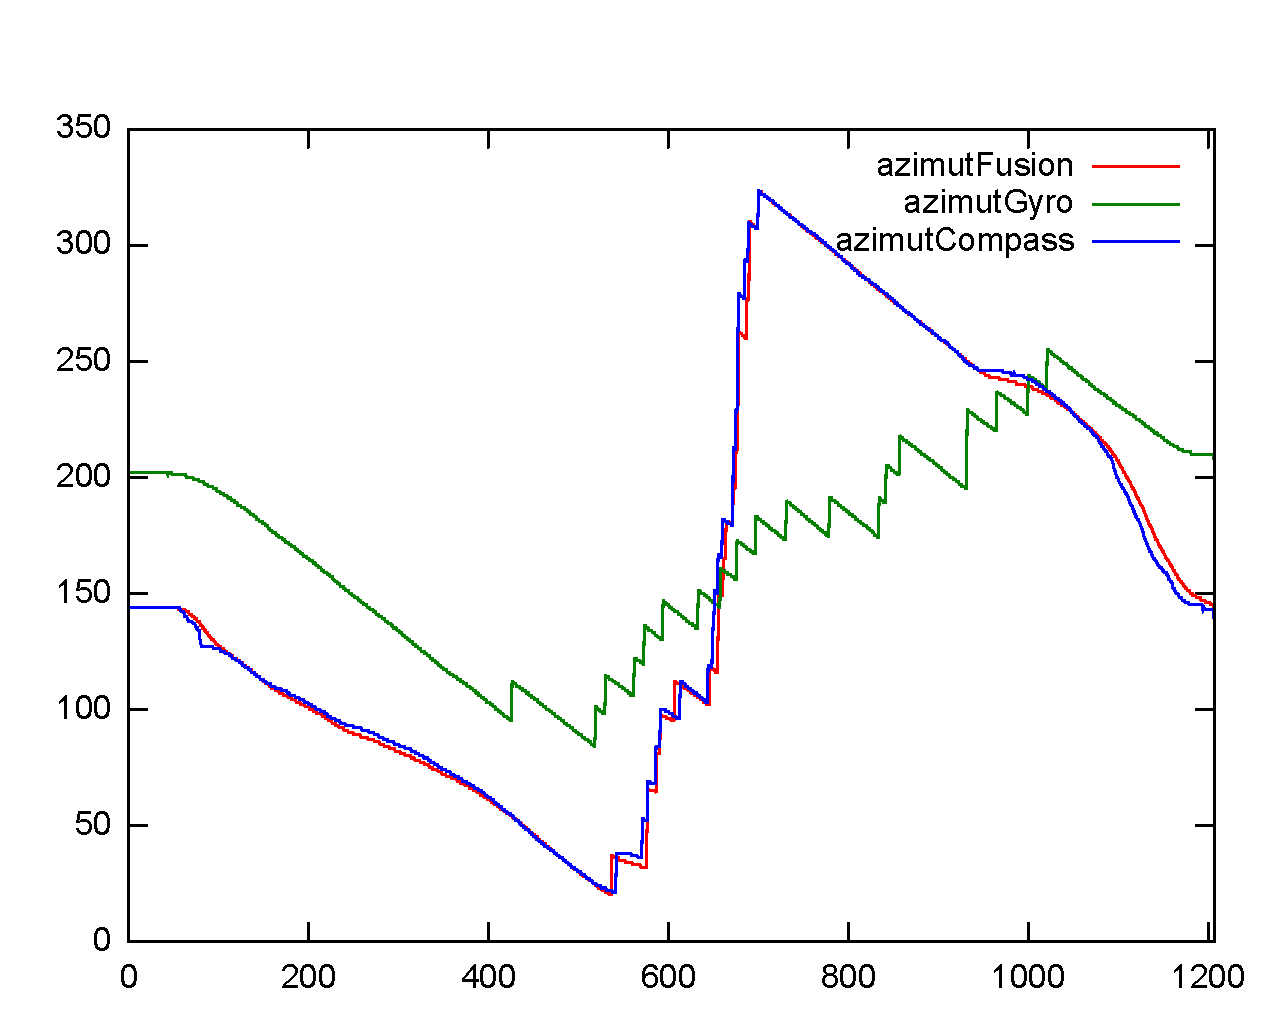
\includegraphics[width=\textwidth]{figures/heading005}
\caption{Gleichmäßige Bewegung in einer Kreisbahn}
\label{fig:heading005}
\end{figure}

Um verlässlichere Aussagen machen zu können habe ich mehrere gleichartige Messungen durchgeführt und dann die Durchschnittswerte verglichen. Bei diesen Messungen wurde ein iPhone 4S mit iOS 5 verwendet. Pro Messung wurde eine Kreisbahn abgefahren und die drei Azimut-Werte wurden aufgezeichnet. Grafik \ref{fig:heading005} zeigt den Mittelwert aus 20 Messungen. Die Zacken in den Linien in der Mitte ist der Tatsache geschuldet, dass der Sprung von 0$^o$ zu 360$^o$ nicht bei jeder Messung zur selben Zeit stattfindet. Darum kommen im Schnitt solche starken Sprünge zu Stande. Diese sollen aber in der Beurteilung nciht weiter stören. Es ist zu erkennen, dass der Kompass (blau) wie oben Erwähnt Sprünge liefert. Dies ist aber durch die Mittelung über 20 Messungen stark abgeschwächt. Trotzdem ist besonders zwischen $0$ und $200ms$, sowie zwischen $1000$ und $1200ms$ ein unterschiedlicher Charakter der Linien zu erkennen. Die rote Linie der Sensorfusion ist deutlich weicher und gleichmäßiger. Die Sprünge des Kompasses sind in Grafik \ref{fig:heading006} sehr gut zu erkennen (grüne Linie). Dies ist wieder eine Visualisierung einer einzigen Messung. Die Sprünge sind bei jeder Messung unterschiedlich, so, dass sich kein aussagekräftiger Durchschnittswert als Grafik darstellen lässt. Der Verlauf der Linien des Kompass-Azimut-Werts aller 20 Messungen entspricht aber in seiner Intensität Grafik \ref{fig:heading006}. Teilweise bleibt der Kompass regelrecht bei einem Wert \emph{hängen}. Genau diese Fehler werden mit der Sensorfusion (rot) sehr erfolgreich ausgeglichen.

\begin{figure}[htb]
\centering
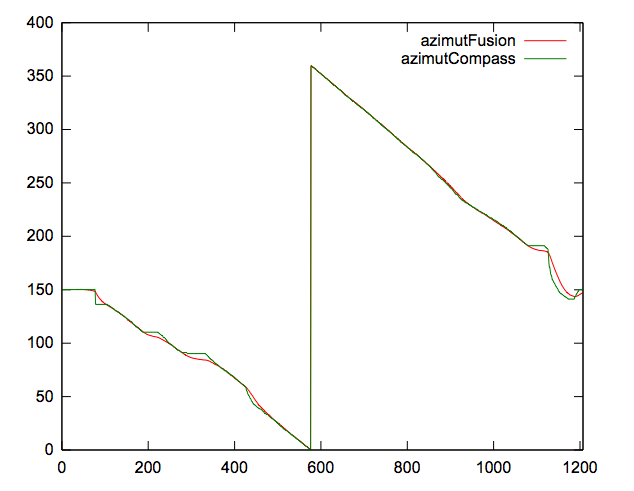
\includegraphics[width=\textwidth]{figures/heading006}
\caption{Sprunghafte Kompasswerte}
\label{fig:heading006}
\end{figure}

\begin{figure}[htb]
\centering
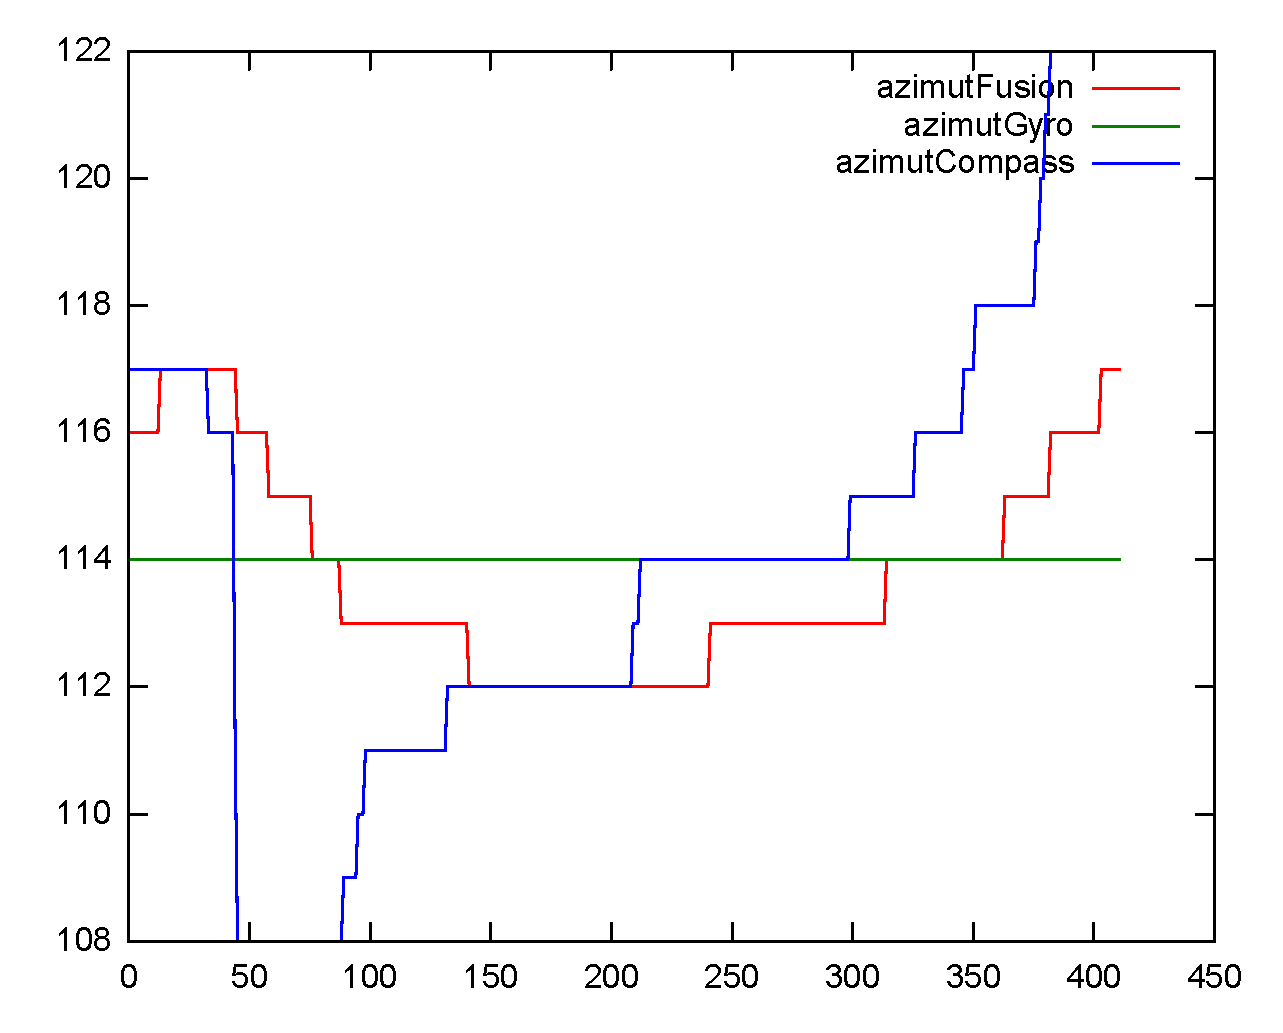
\includegraphics[width=\textwidth]{figures/heading007}
\caption{Störfeld}
\label{fig:heading007}
\end{figure}
Auch Messungen mit Störfeld wurden durchgeführt. Grafik \ref{fig:heading007} zeigt den Durchschnitt von fünf Messungen. Hierbei wurde an dem ruhenden iPhone ein Störfeld vorbei geführt. Schön ist zu erkennen, dass sich das Gyroskop (grün) völlig ruhig, also korrekt, verhält. Die kurzzeitige Magnetfeldstörung findet zwischen $40$ und $100ms$ statt. Der Azimut-Wert des Kompass (blau) springt von einer Messung zur nächsten im Schnitt 8 Grad auf einmal. Die Sensor-Fusion (rot) kann diese Deviation etwas ausgleichen. Jedoch schwankt die rote Linie trotzdem noch etwas. Es ist aber zu beachten, dass die Werte der Sensor-Fusion Maximal $3^o$ abweichen und die des Kompass gleich $6^o$. %Die mittlere Abweitung der Sensor-Fusion beträgt $^o$ und die des Kompasses $^o$.
Der hier verwendete Fusions-Algorithmus kann allerdings nur kurze Magnetfeld-Störungen ausgleichen. Diese kommen häufiger vor als länger andernde. Zum Beispiel durch Mobiltelefone und sonstige Funkwellen. Dieser Fusions-Algorithmus ist dazu gedacht das visuelle Erscheinungsbild weicher, also angenehmer und natürlicher, zu gestalten.

Es bleibt festzuhalten, dass zu Beginn meiner Arbeiten gerade erst das iPhone 4 erschienen war und zum ersten mal ein Gyroskop in einem iOS-Gerät verbaut war. Das iPad 2, mit dem wir hauptsächlich arbeiteten, hatte nochmals ein leicht anderes Gyroskop-Modell als das iPhone 4 verbaut. Damals war zusätzlich iOS 4 ziemlich frisch erschienen. Zum ersten mal konnten über die CoreMotion API Gyroskop-Daten ausgelesen werden. Die Apple-eigene Sensorfusion war daher noch sehr unausgereift. Inzwischen sind 1,5 Jahre vergangen, iOS 6 steht in den Startlöchern. Meine letzten Entwicklungsschritte fanden bereits unter iOS 6 statt. In dieser Zeit haben sich Augmented Reality Apps als Erweiterung besteheneder Angebote etabliert. Apple selbst hat ebenfalls merklich Entwicklungsarbeit für die CoreMotion API aufgewendet. Der Kompass ist weitaus weniger sprunghaft und auch viel weniger anfällig auf Magnetfeld-Störungen. Apple hat quasi teilweise im selben Gebiet weiterentwickelt wie ich. Das ist technischer Fortschritt. Trotzdem ist es weiterhin sinnvoll nicht ausschließlich auf den Kompass-Wert der CoreMotion API zu vertrauen. Dieser ist immernoch sprunghaft, wenngleich dies auch viel minimaler ausfällt als noch vor einigen Monaten. 

Trotz des relativ einfachen Verfahrens, welches nur etwas Feinjustierung hinsichtlich der jeweiligen Hardware nötig hat, kann ein brauchbares Ergebnis erzielt werden. Wenn die verfügbaren Sensoren richtig kombiniert werden sind die Resultate sehr stabil. Daran haben auch die Verfahren Teil die Apple schon in seinen Cocoa touch Frameworks anwendet. Leider hat man darin keinen Einblick als einfacher Entwickler. Apple erläutert an keiner Stelle der API-Dokumentation wie die Daten die die API ausgibt zustande kommen. Die errechnete Orientierung ist praxistauglich und kann in jede iOS-App einfach implementiert werden. Das Ergebnis sieht aus wie in Abbildung \ref{fig:ipad-navi}

\begin{figure}[htb]
\centering
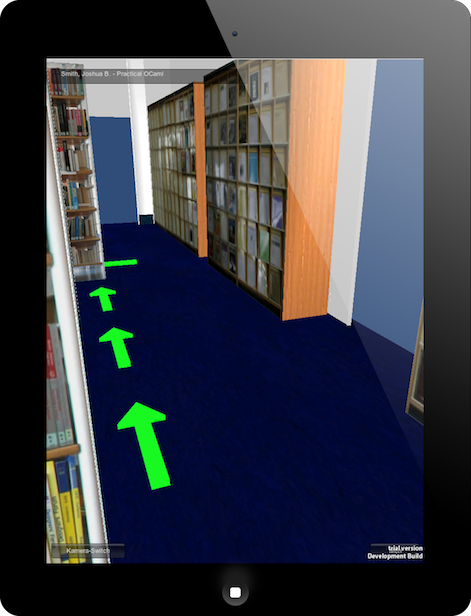
\includegraphics[scale=0.83]{figures/ipad-navi}
\caption{Fertige Ansicht des 3D-Modells in der App}
\label{fig:ipad-navi}
\end{figure}